\part{Ejercicio 1}
\section{Enunciado}
Dado un n'umero natural n mayor que 1, encontrar el n'umero primo $p$ que aparece con mayor potencia en la factorizaci'on 
de n. En caso de haber m'as de un n'umero primo con  la mayor potencia, encontrar el mayor de ellos.

%TODO: revisar la claridad de esto, ver si se puede mejorar
\section{Desarrollo}
La primer idea para resolver el ejercicio fue obtener los primos menores que el n'umero a factorizar
(en adelante $n$) y luego obtener la potencia con la que cada uno lo divide, qued'andonos con el de mayor
potencia o con el mayor de todos los de m'axima potencia. Sin embargo esta soluci'on era costosa, ya que
requer'ia obtener primeramente todos aquellos primos que sean menores a $n$.
\paragraph{}
Un segundo acercamiento nos permiti'o salvar esta dificultad, de manera que no fue necesario obtener 
los primos menores a $n$ expl'icitamente. El proceso consiste en partir de 2, probar manualmente si 2, 3 y 5 
dividen a $n$ y a partir  de aqu'i ciclar generando n'umeros de la forma $6*k + 1$ o $6*k + 5$ con $k \geq 1$ 
(se puede demostrar que los n'umeros primos mayores que 5 tienen esta forma (ver Demostraci'on 1)).
\paragraph{}
Cuando hallamos alg'un n'umero primo que divide a $n$, buscamos su multiplicidad dividiendo nuestro n'umero 
por dicho primo, tantas veces como sea posible. Una vez calculada, se verifica si esta nueva multiplicidad 
es mayor a la guardada hasta el momento. Si lo es, 'esta es reemplazada por la nueva. Una vez hecho esto 
se pasa al siguiente posible primo, repitiendo el proceso anterior pero ahora con un nuevo $n$ que llamaremos 
$n'$, y que resulta de dividir $n$ por el n'umero primo, elevado a la potencia hallada. Este proceso se repite 
mientras nuestro pr'oximo primo no supere la ra'iz de $n'$. Un problema de este m'etodo es que se hacen 
divisiones por n'umeros que no son primos, pero su costo es menor compar'andolo con otras metodolog'ias que
buscan todos los primos menores a $n$, o que verifican si dicho n'umero lo es antes de hacer la divisi'on.
\paragraph{}
Es importante notar que si un n'umero no es primo, este no puede dividir a $n$ (ver demostraci'on 2). Si 
no se pudiera asegurar esto, el algoritmo fallar'ia. Un ejemplo simple seria al factorizar $30 = 2*3*5$. 
En este caso se guardar'ia a 15 como m'aximo factor primo, lo cual resulta claramente err'oneo. Finalmente, 
utilizamos un teorema que nos dice que si un n'umero es compuesto existe por lo menos un primo menor que su 
ra'iz cuadrada que lo divide (ver demostraci'on 3), lo que nos permite iterar solo hasta la ra'iz del n'umero 
(la cual se actualiza luego de terminada la divisi'on) en vez de hasta $n$.

\section{Demostraciones}
\subsection{Teorema 1}
\paragraph{Enunciado:}
Sea p $\in$ $\enteros$, primo , p $>$ 5, entonces $\exists$ k $\in$ $\enteros$ $\geq$ 1  tal que p = $6*k+1$ o p = $6*k +5$.
\paragraph{Demostraci'on:}
Lo demostraremos por absurdo.\\ 
Supongamos que $\exists$ p $\in$ $\enteros$, primo, tal que p $>$ 5 y p $\not\equiv$ 1  $\mod{6}$ y p
$\not\equiv$ 5  $\mod{6}$, luego p = $6*k + j$ con j $\in$ ${0,2,3,4}$ \\
si $j = 0$\\
$6*k$ $\equiv$ 0  $\mod{6}$, absurdo pues p es primo\\
si $j = 2$\\
$6*k + 2$ $\equiv$ 0  $\mod{2}$, absurdo pues p es primo \\
si $j = 3$\\
$6*k + 3$ $\equiv$ 0  $\mod{3}$, nuevamente absurdo\\
si $j = 4$\\
$6*k + 4$ $\equiv$ 0  $\mod{2}$, tambi'en llegamos a un absurdo.\\
Ergo, si p es primo y p $>$ 5, entonces p = $6*k+1$ o p = $6*k +5$.

\subsection{Teorema 2}
\paragraph{Enunciado:}
Sea k $\in$ $\enteros$ compuesto, y sea n $\entero$ para todo p $\entero$ primo, p $<$ k, $(n:p) = 1$, entonces n $\not\equiv$ 0 $\mod{k}$
\paragraph{Demostraci'on}
Dado que k es compuesto existen $q_1,\ldots,q_j$ con $q_i$ primo tal que $q_1*\ldots*q_j = k$ \\
Supongamos que n $\equiv$ 0 $\mod{k}$,\\
Entonces como los $q_i$ son primos, vale que n $\equiv$ 0 $\mod{q_1}$ 'o ... 'o $n \equiv 0 \mod{q_j}$ \\
Pero sabemos que $q_i < k$ y que por lo tanto $(n:q_{i}) = 1$ \\
Llegamos entonces a un absurdo que provino de suponer que  $n \equiv 0 \mod{k}$ \\ 
Luego $n \not\equiv 0 \mod{k}$, que era lo que quer'iamos probar.

\subsection{Teorema 3}
\paragraph{Enunciado:}
$k$ $\entero$, $k>1$; $k$ es compuesto $\longleftrightarrow$ $\exists p$ primo tal que $p \leq \sqrt{k}$ y $k \equiv 0 \mod{p}$
\paragraph{Demostraci'on:}
Analizamos por separado las dos implicaciones: \\
$\leftarrow)$ trivial \\
$\rightarrow$) Como $k$ es compuesto se puede factorizar como $p_1*...*p_n$ con $p_i > \sqrt{k} \forall i \in {1...n}$\\
Entonces \\
$k = p_1*...*p_n > (\sqrt{k})^2*T$ , con $T>1$\\  
$k = p_1*...*p_n > \sqrt{k}^2*T$ pero $k*T > k$ \\
Absurdo, que provino de suponer que $p_i > \sqrt{k}$ $\forall i \in {1...n}$.\\

%TODO: hacer el cambio al pseudocodigo para q sea mas facil la demo
\section{Pseudoc'odigo}
\begin{algorithm}
\caption{Halla $mejorPrimo$ y $mejorPotencia$}
\begin{algorithmic}[1]
\STATE $mejorPrimo \leftarrow 1$
\STATE $mejorPotencia \leftarrow 0$
\STATE $primoActual \leftarrow generar\_candidato()$
\STATE $potenciaActual \leftarrow 0$
\STATE $l \leftarrow limite(n)$
\WHILE{$n \neq 1$ $\&$ $primoActual \leq l$}
    \IF{$primoActual$  $|$ $n$}
        \STATE $potenciaActual++$
        \STATE $n \leftarrow n/primoActual$
    \ELSE
        \IF{$potenciaActual \geq mejorPotencia$}
            \STATE $mejorPrimo \leftarrow primoActual$
            \STATE $mejorPotencia \leftarrow potenciaActual$
        \ENDIF

        \STATE $potenciaActual \leftarrow 0$
        \STATE $primoActual \leftarrow generar\_candidato()$
        \STATE $l \leftarrow limite(n)$
    \ENDIF
\ENDWHILE
\IF{$primoActual > l$}
    \STATE $primoActual \leftarrow n$
    \STATE $potenciaActual \leftarrow 1$
\ENDIF
\IF{$potenciaActual \geq mejorPotencia$}
    \STATE $mejorPrimo \leftarrow primoActual$
    \STATE $mejorPotencia \leftarrow potenciaActual$
\ENDIF
\end{algorithmic}
\end{algorithm}


%En el pseudoc'odigo presentado se utilizan dos funciones auxiliares:
En el pseudoc'odigo presentado se utiliza una funcion auxiliar:
\begin{itemize}
%\item $limite(n)$ es una macro para $\lceil\sqrt{n}\rceil$
\item $generar\_candidato()$ es un procedimiento tipo $factory$ que conserva un estado interno 
y genera candidatos a n'umeros primos como se describi'o en el Teorema 1
\end{itemize}

%TODO: hablar del calculo de complejidad, de porq logaritmico, hacer el calculo
%TODO: analisis de peor caso!
\section{C'alculo de complejidad}
\paragraph{}
En este ejercicio usamos el modelo logar'itmico de complejidad ya que la entrada del problema es 'unicamente un
n'umero entero y el grueso de las operaciones involucradas son 'unicamente sentencias de control de flujo
y operaciones aritm'eticas sobre enteros. En funci'on de esto no ser'ia l'ogico despreciar el aumento del costo
de operar sobre dichos n'umeros a medida que la entrada crece.

\paragraph{}
A partir del pseudoc'odigo se puede identificar r'apidamente el bucle principal donde se realizan la mayor'ia
de las operaciones. Veamos primero el c'odigo fuera del bucle.
\begin{itemize}
\item $limite(n)$ tiene un costo $O(log^3 n)$, puesto que la operaci'on m'as costosa que realiza es una ra'iz
cuadrada, y la complejidad de dicha operaci'on es la m'as importante. En este caso $n$ es una variable que contiene
inicialmente el valor del par'ametro de entrada y a lo largo de la ejecuci'on se divide en sucesivas ocasiones, por
lo tanto su valor decrece y est'a acotado por el valor inicial.
\item $generar\_candidato()$ tiene un costo $O(log^2 n)$ ya que para casos grandes solo efect'ua un chequeo de
una variable booleana y una multiplicaci'on de un entero acotado por $n$.
\end{itemize}
El resto de las operaciones realizadas antes y después del bucle tienen una complejidad de a lo sumo $O(log$ $n)$,
y por lo tanto son despreciables respecto del orden predominante que es hasta el momento $O(log^3 n)$ si no tenemos
en cuenta al ciclo principal.

\paragraph{}
Observemos ahora el comportamiento de dicho bucle. Se demostrará a continuaci'on que este bucle se ejecuta a lo sumo
$O(\sqrt{n})$ veces, pero por el momento veamos la complejidad del c'odigo contenido en el mismo. Si observamos
l'inea por l'inea el pseudoc'odigo puede verse que el cuerpo del ciclo es una sucesi'on de operaciones aritm'eticas,
donde la más costosa es la multiplicaci'on, cuya complejidad es $O(log^2 n)$.

\paragraph{}
Resta entonces demostrar que el ciclo itera a lo sumo $O(\sqrt{n})$ veces. Si analizamos la guarda del ciclo vemos
que se trata de una conjunci'on booleana. Con que cualquiera de las dos formulaciones booleanas sea falsa, el ciclo
termina y el algoritmo se finaliza en tiempo constante. Para que esto ocurra, alcanza con que $n = 1$ o $primoActual^2
> limite$ o equivalentemente $primoActual > \sqrt{limite}$. Represento por $nombre_i$ el valor de la variable $nombre$ 
en la iteraci'on $i$. 

\paragraph{}
Al entrar al ciclo hay dos casos posibles: o bien $primoActual$ $|$ $n$, o no lo hace. Llamemos a estas dos
posibilidades caso 1 y caso 2 respectivamente, y analicemos por separado.
%FIXME: queda demasiado espacio aca!
\begin{itemize}
\item Caso 1: $primoActual$ $|$ $n$ \\
En este caso se divide a $n$ por $primoActual$ mientras sea posible. Como $primoActual \geq 2$, resulta
sencillamente que la cantidad de veces que puede ejecutarse este bloque es $O(log_2 n)$. Necesariamente
despu'es de esa cantidad de iteraciones tendremos $n = 1$ y el ciclo termina.
\item Caso 2: $primoActual \nmid n$\\
En este otro caso se cumple que $\forall n > N$, $primoActual_{i+1} \geq primoActual_i + 1$. Esto se deduce
por construcci'on del procedimiento $generar\_candidatos()$ que produce una sucesi'on de la forma: \\

\centerline{2, 3, 5, 6 * 1 + 1, 6 * 1 + 5, 6 * 2 + 1, 6 * 2 + 5, 6 * 3 + 1, 6 * 3 + 5 ...} 

Si adem'as vemos que en este caso $primoActual_{i+1}$ es el t'ermino de la sucesi'on que est'a 
inmediatamente a continuaci'on de $primoActual_i$. Por consiguiente $primoActual$ crece
de forma tal que supera el valor de $\sqrt{limite}$ en $O(\sqrt{limite})$ iteraciones (puesto
que $primoActual > 0$ en todo momento, $|$ $primoActual - \sqrt{limite}$ $|$ $< \sqrt{limite}$).
Además resulta claro que $limite \leq n$ ya que su valor inicial es $n$ y luego decrece
progresivamente.
\end{itemize}

\paragraph{}
Finalmente vemos que el caso 1 resulta en a lo sumo $O(log_2 n)$ iteraciones, mientras que
el caso 2 resulta en $O(\sqrt{n})$. Por lo tanto la totalidad de iteraciones es:\\
\\
\centerline{$O(log_2 n + \sqrt{n}) = O(\sqrt{n})$}
\paragraph{}
Y el orden de complejidad del ciclo teniendo en cuenta el costo de cada iteraci'on es por lo tanto:\\
\\
\centerline{$O(log^2 n \sqrt{n})$}
\paragraph{}
Siendo $n$ el valor del entero que el algoritmo toma como par'ametro. Por otra parte sabemos que 
el tamaño en memoria de un entero arbitrario $n$ es $t = log_2 n$, por lo tanto:\\
\\
\centerline{$2^t = n \Rightarrow \sqrt{n}$ $log^2 n = 2^t$ $t^2$}
\\
\paragraph{}
Finalmente pudimos demostrar que $T(t) \in O(2^t $ $t^2)$.


%TODO: hablar de que sabemos q n no es tam de entrada, que dejamos los graficos porq se ve bien el o(sqrtn), ojo con esto q me parece q es O(raiz*log^3)
\section{An'alisis Experimental}
\subsection{Experiencias realizadas}
Para el an'alisis del algoritmo decidimos medir tanto operaciones como tiempo. Primero medimos dichas variables 
para los n'umeros entre 2 y 100000 para observar un patr'on de comportamiento. A partir de esta experiencia, 
decidimos realizar otras dos, donde separamos n'umeros primos en una de ellas, y en la otra tomamos las potencias 
de un n'umero primo (en particular de 7). Esto lo hicimos por considerar que el peor caso del algoritmo es 
precisamente cuando el n'umero es primo, mientras que el mejor caso es cuando el n'umero es potencia de un primo. 
Por otro lado realizamos experiencias similares pero teniendo en cuenta ya no el numero, sino la cantidad de bits 
de su representaci'on binaria, es decir teniendo en cuenta el tama\~{n}o de la entrada. Para estas experiencias 
tomamos distintos n'umeros pero medimos la cantidad de operaciones y el tiempo en funci'on de $\lfloor log_2(n) \rfloor + 1$.

\subsection{Gr'aficos}
\subsubsection{Gr'aficos en funcion de n}

\begin{figure}[H]
\centering
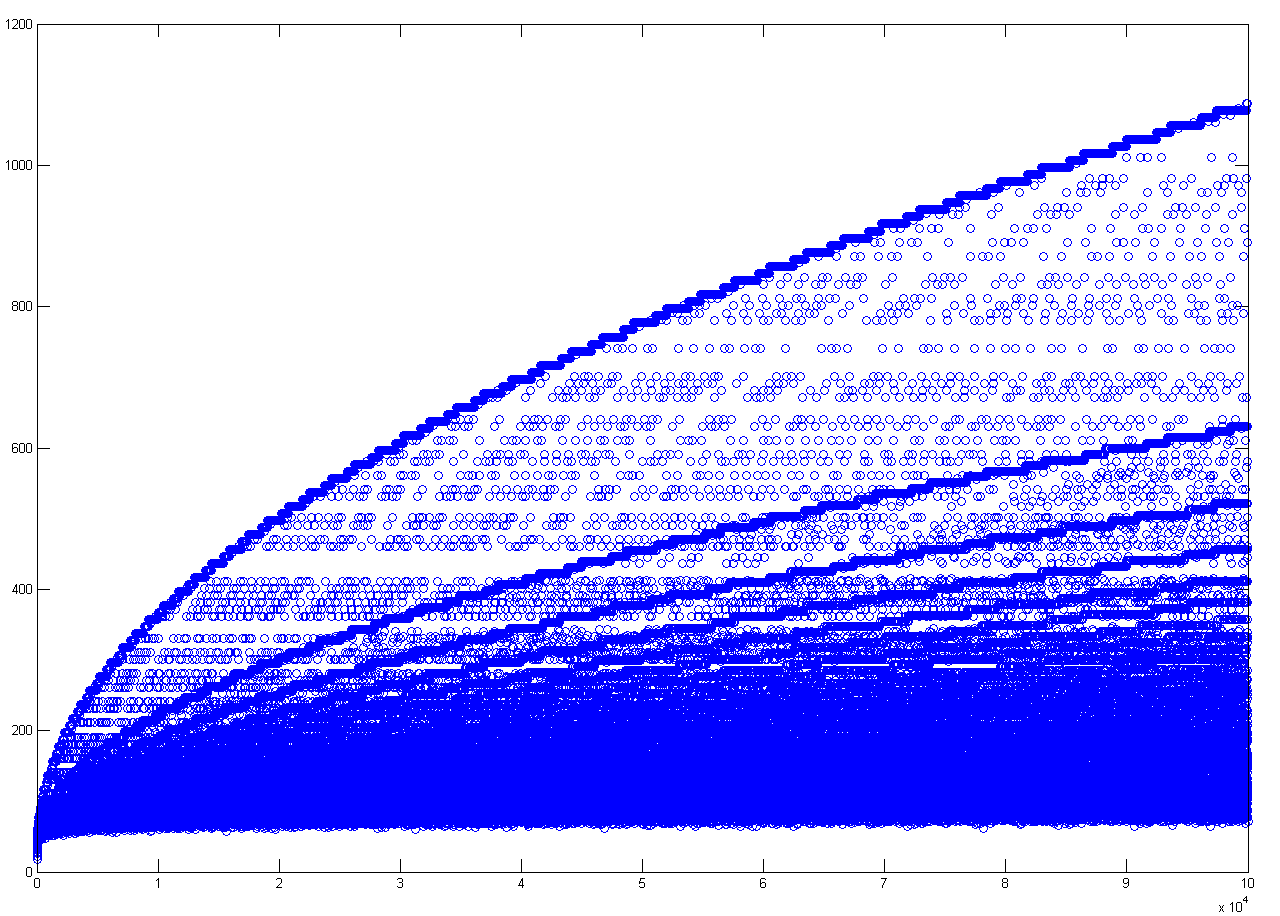
\includegraphics[scale=0.7]{../../codigo/ejercicio1/benchmark/graficos/todos_los_numeros/graficosTodos.png}
\caption{Cantidad de operaciones en funci'on de $n$}
\end{figure}

\begin{figure}[H]
\centering
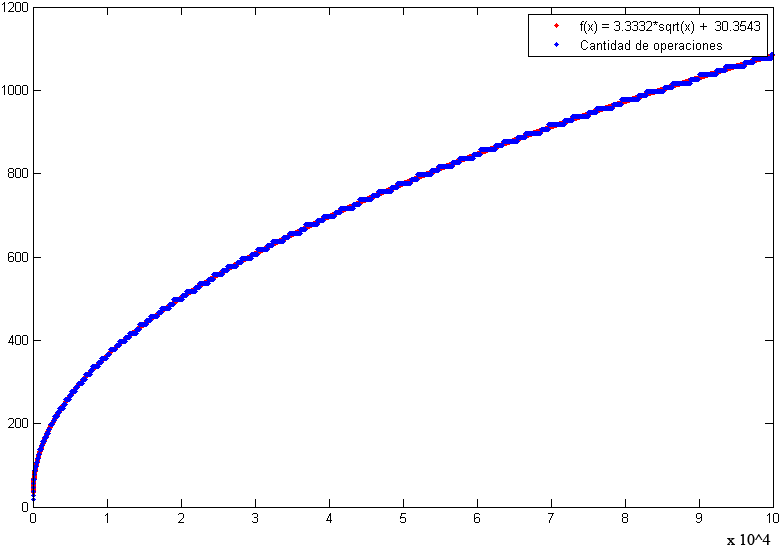
\includegraphics[scale=0.8]{../../codigo/ejercicio1/benchmark/graficos/primos/graficoPrimos.png}
\caption{Cantidad de operaciones en funci'on del $n$ para $n$ primo}
\end{figure}

\begin{figure}[H]
\centering
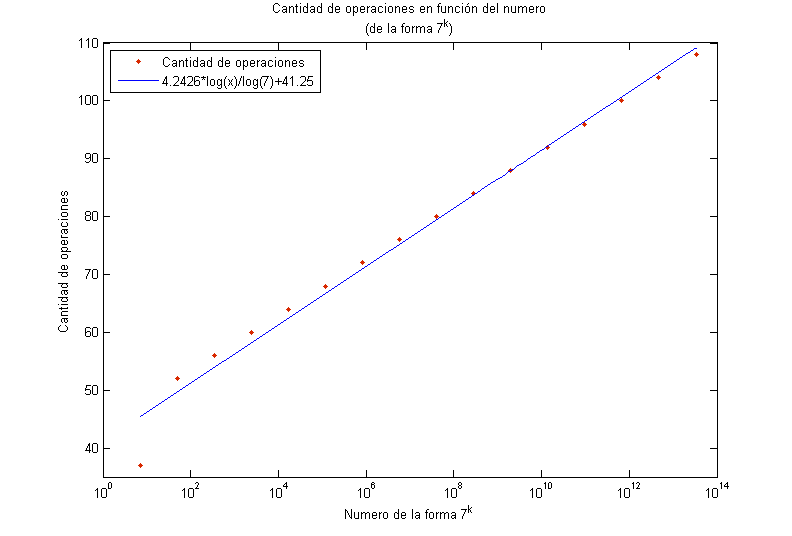
\includegraphics[scale=0.8]{../../codigo/ejercicio1/benchmark/graficos/potencias_de_7/graficoPotenciasDe7.png}
\caption{Cantidad de operaciones en funci'on de $n$ para $n$ de la forma $7^k$}
\end{figure}

\begin{figure}[H]
\centering
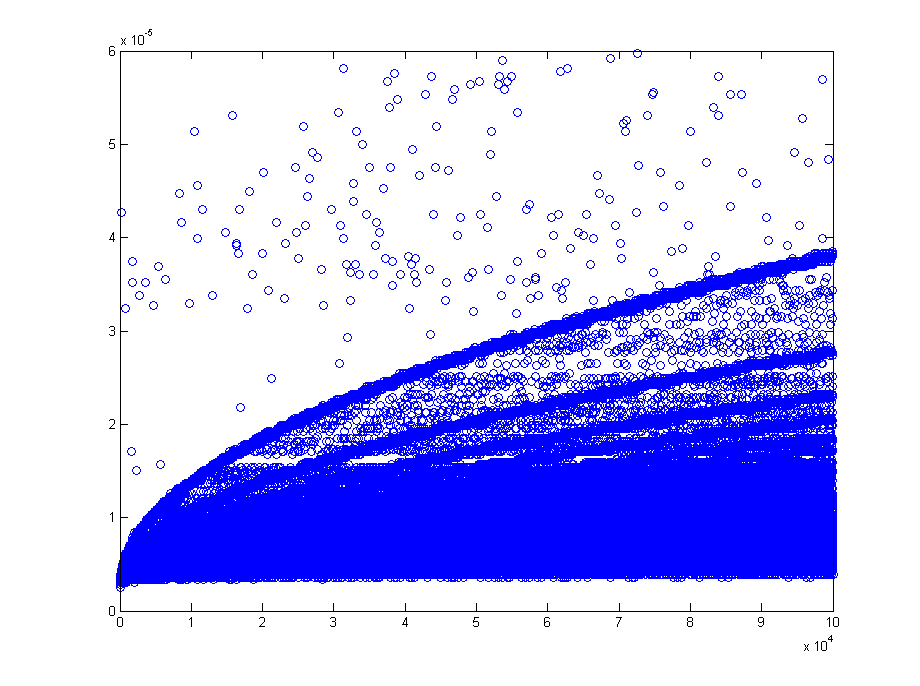
\includegraphics[scale=0.5]{../../codigo/ejercicio1/benchmark_de_tiempo/graficos/todos_los_numeros/todosLosNumerosPuntosTiempo.png}
\caption{Tiempo en funci'on de $n$}
\end{figure}

\subsubsection{Gr'aficos en funcion del tama\~{n}o de la entrada}
\begin{figure}[H]
\centering
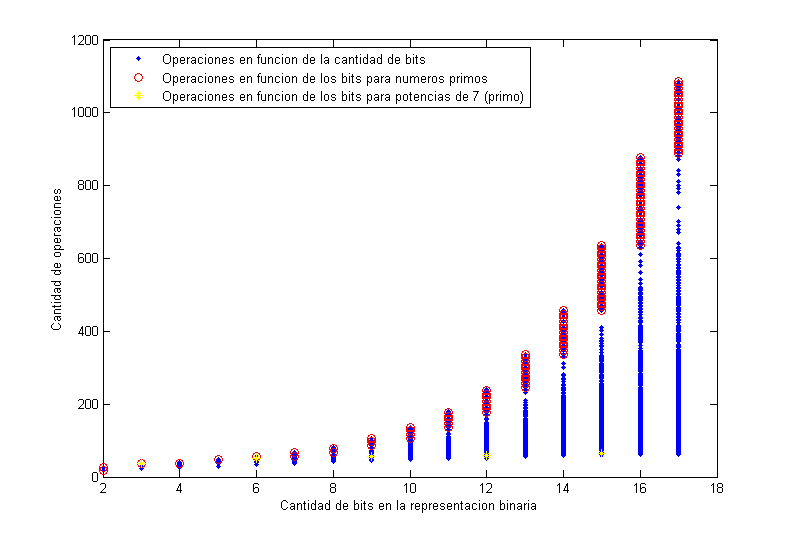
\includegraphics[scale=0.7]{../../codigo/ejercicio1/benchmark/graficos/tamanio_Entrada_T/operacionesEntrada.png}
\caption{Cantidad de operaciones en funci'on del tama\~{n}o de la entrada}
\end{figure}

\begin{figure}[H]
\centering
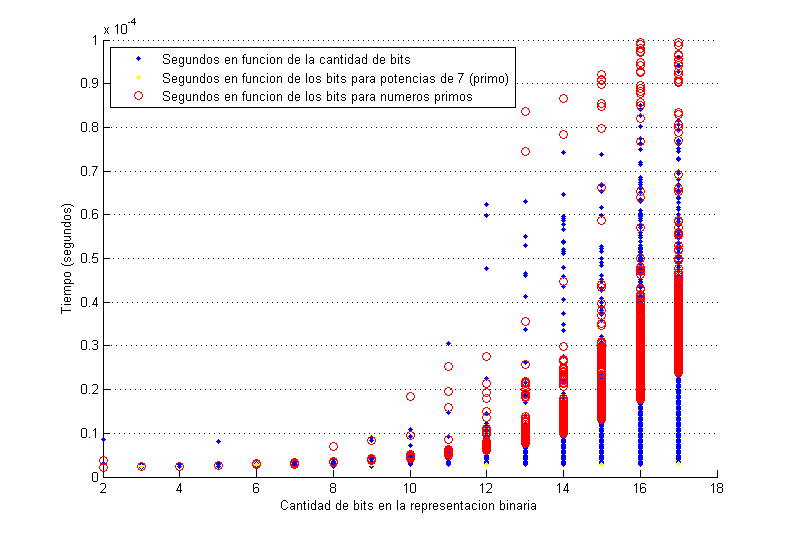
\includegraphics[scale=0.7]{../../codigo/ejercicio1/benchmark_de_tiempo/graficos/tamanio_Entrada_T/Tiempo_en_funcion_bits.png}
\caption{Cantidad de operaciones en funci'on del tama\~{n}o de la entrada}
\end{figure}

\section{Discusi'on}
En los gr'aficos pudimos observar lo que el an'alisis te'orico nos anunci'o.

En la figura 1, se ve claramente como existen diversos patrones de comportamiento. As'i el techo es un funci'on del tipo ra'iz 
cuadrada, mientras que debajo se encuentran otras funciones de orden logar'itmico. Esta situaci'on se ve mas claro en los 
gr'aficos donde solo est'an los n'umeros primos y las potencias de 7. En ambos casos pudimos, mediante cuadrados m'inimos, 
encontrar una funci'on que se asemeje al comportamiento de las muestras, lo cual refuerza nuestra idea de mejor y peor caso.\\
El gr'afico en funci'on del tiempo muestra un comportamiento muy similar al gr'afico de cantidad de operaciones, pero presenta 
$outliers$ que se pueden explicar por el hecho de que tomar tiempos esta sujeto a un error de medici'on producto del uso del sistema
de pruebas por parte de otros procesos.

A la hora de analizar los gr'aficos en funci'on del tama\~{n}o de la entrada esperamos ver g'raficos con forma exponencial 
y fue exactamente eso lo que obtuvimos. En el caso de cantidad de operaciones, se mantuvo lo observado en los otros gr'aficos, 
es decir que en general los primos requieren m'as operaciones que el resto de los n'umeros, mientras que las potencias de 7 
requieren muchas menos.

Finalmente la figura 6 mantiene la tendencia, y nuevamente presenta $outliers$ propios de los factores externos que intervienen 
en la medici'on de tiempos.

A modo de conclusi'on podemos afirmar que la experimentaci'on emp'irica valid'o nuestros resultados te'oricos.
